% 3.5V pics
\FloatBarrier

\begin{figure}[h!]
	\centering
	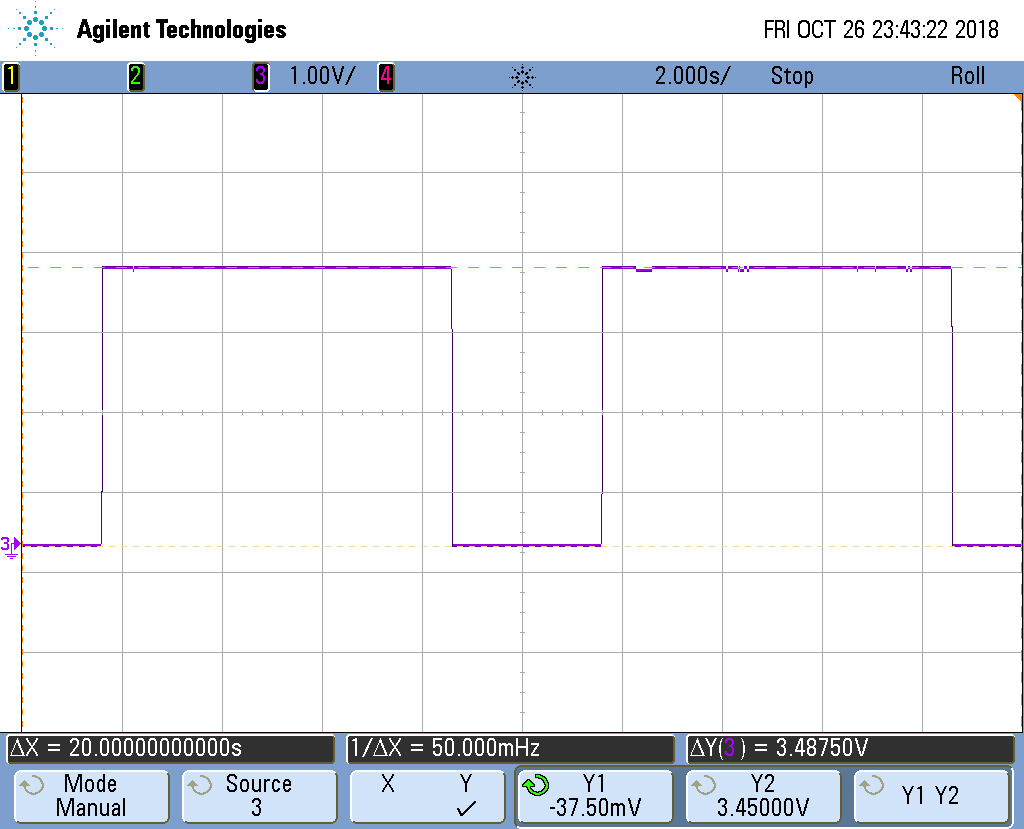
\includegraphics[scale=0.75]{../images/scope_10.png}
	\caption{$V_{in}$ Measurement for $3.5$\si{\volt} Reference}
	\label{fig:scope_10}
\end{figure}

\FloatBarrier

\FloatBarrier

\begin{figure}[h!]
	\centering
	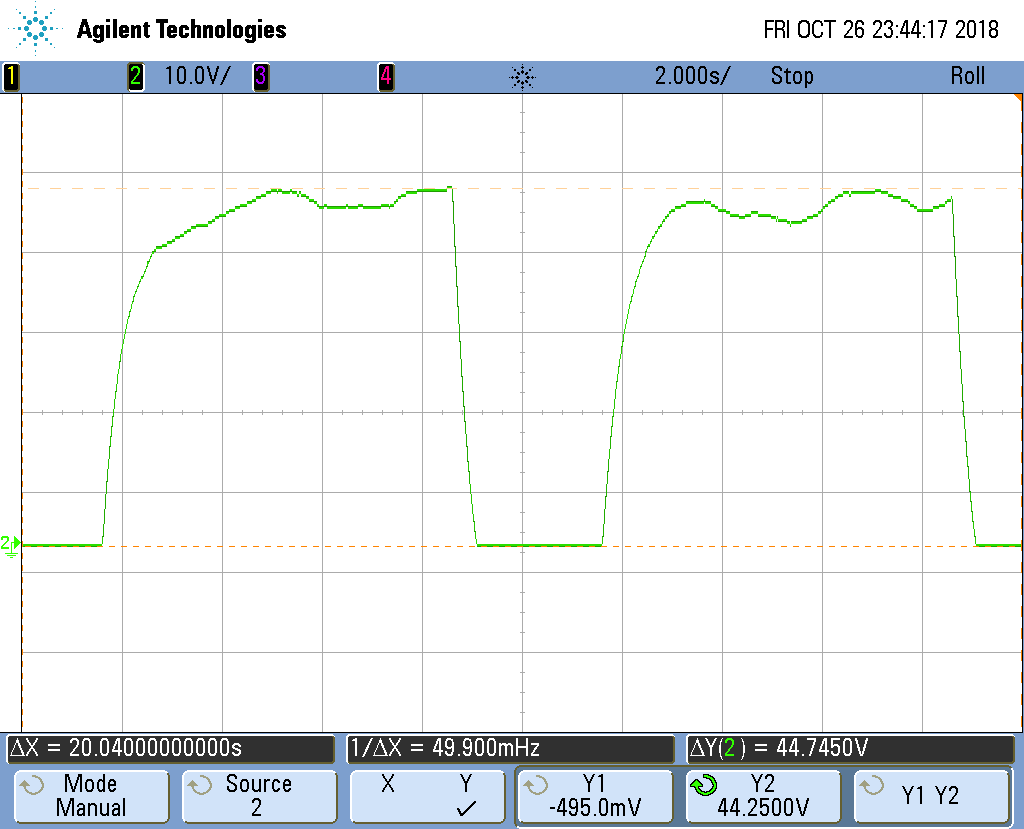
\includegraphics[scale=0.75]{../images/scope_11.png}
	\caption{$V_{out}$ Measurement for $3.5$\si{\volt} Reference}
	\label{fig:scope_11}
\end{figure}

\FloatBarrier

\FloatBarrier

\begin{figure}[h!]
	\centering
	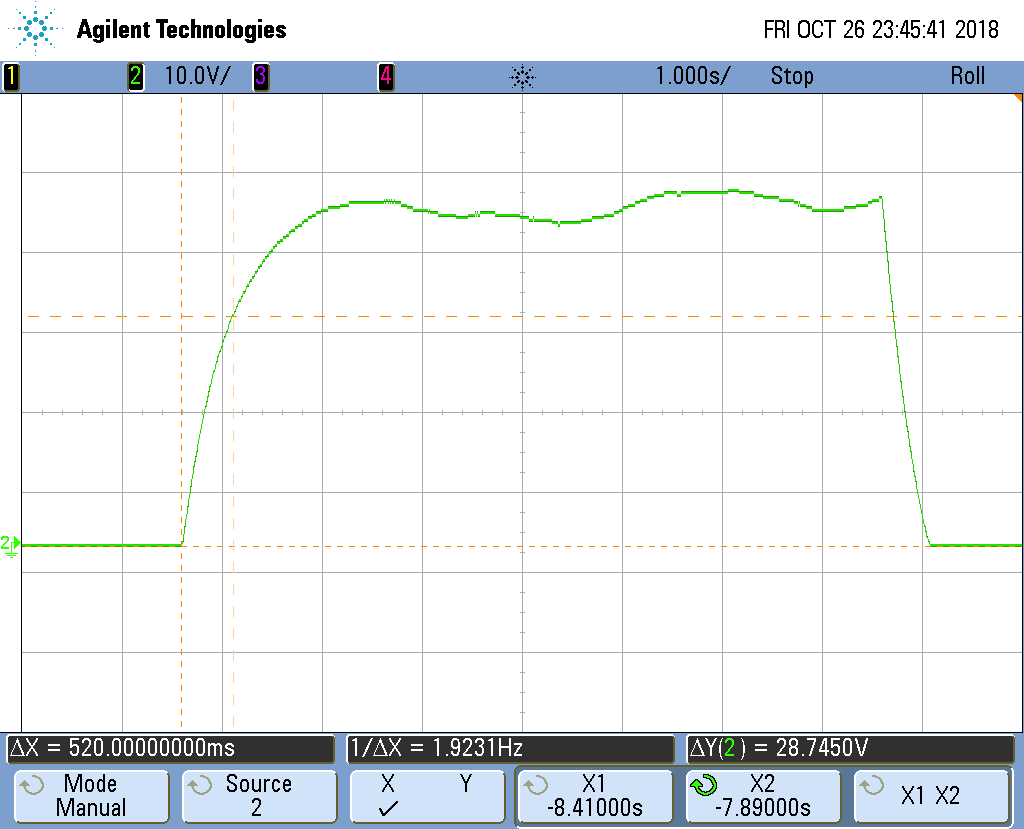
\includegraphics[scale=0.75]{../images/scope_12.png}
	\caption{$\tau$ Measurement for $3.5$\si{\volt} Reference}
	\label{fig:scope_12}
\end{figure}

\FloatBarrier

% 4V pics
\FloatBarrier

\begin{figure}[h!]
	\centering
	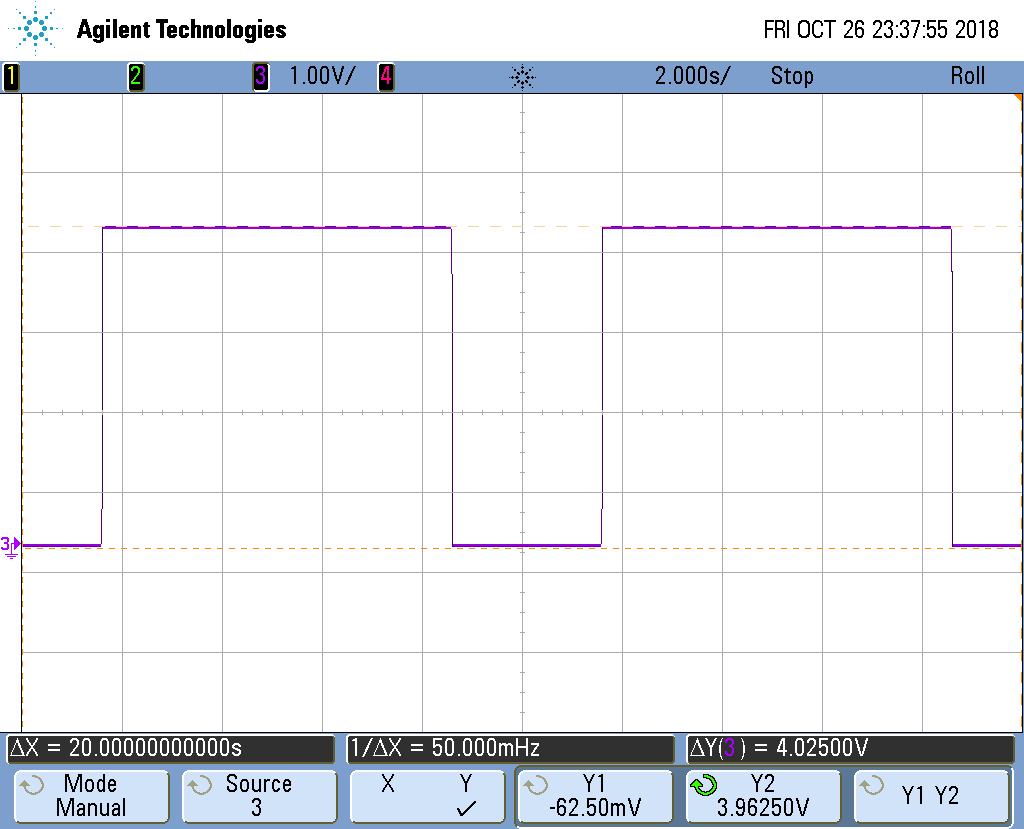
\includegraphics[scale=0.75]{../images/scope_6.png}
	\caption{$V_{in}$ Measurement for $4$\si{\volt} Reference}
	\label{fig:scope_6}
\end{figure}

\FloatBarrier

\FloatBarrier

\begin{figure}[h!]
	\centering
	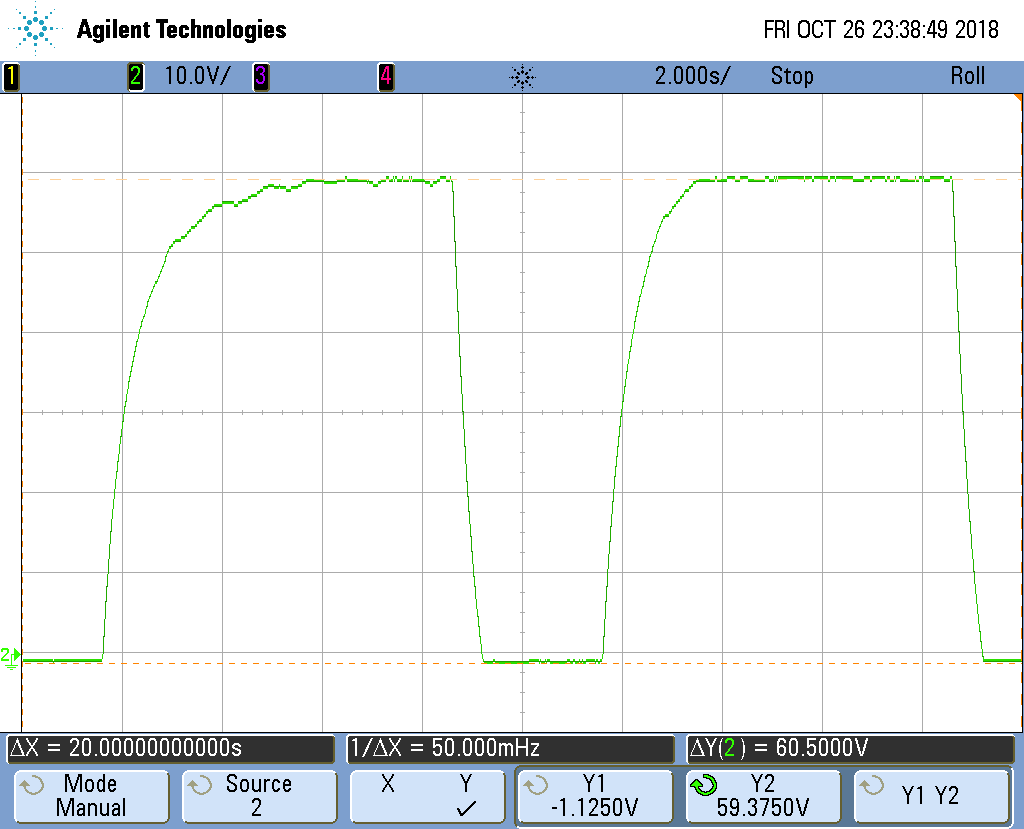
\includegraphics[scale=0.75]{../images/scope_7.png}
	\caption{$V_{out}$ Measurement for $4$\si{\volt} Reference}
	\label{fig:scope_7}
\end{figure}

\FloatBarrier

\FloatBarrier

\begin{figure}[h!]
	\centering
	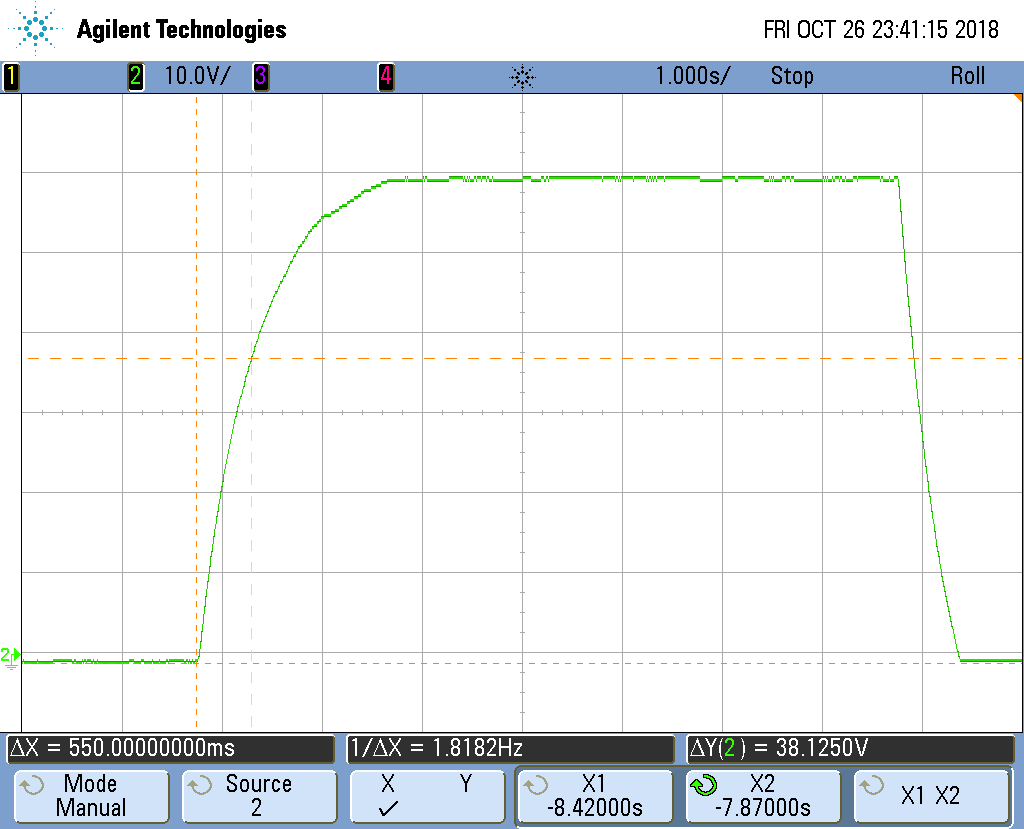
\includegraphics[scale=0.75]{../images/scope_8.png}
	\caption{$\tau$ Measurement for $4$\si{\volt} Reference}
	\label{fig:scope_8}
\end{figure}

\FloatBarrier

% 4.5V pics

\FloatBarrier

\begin{figure}[h!]
	\centering
	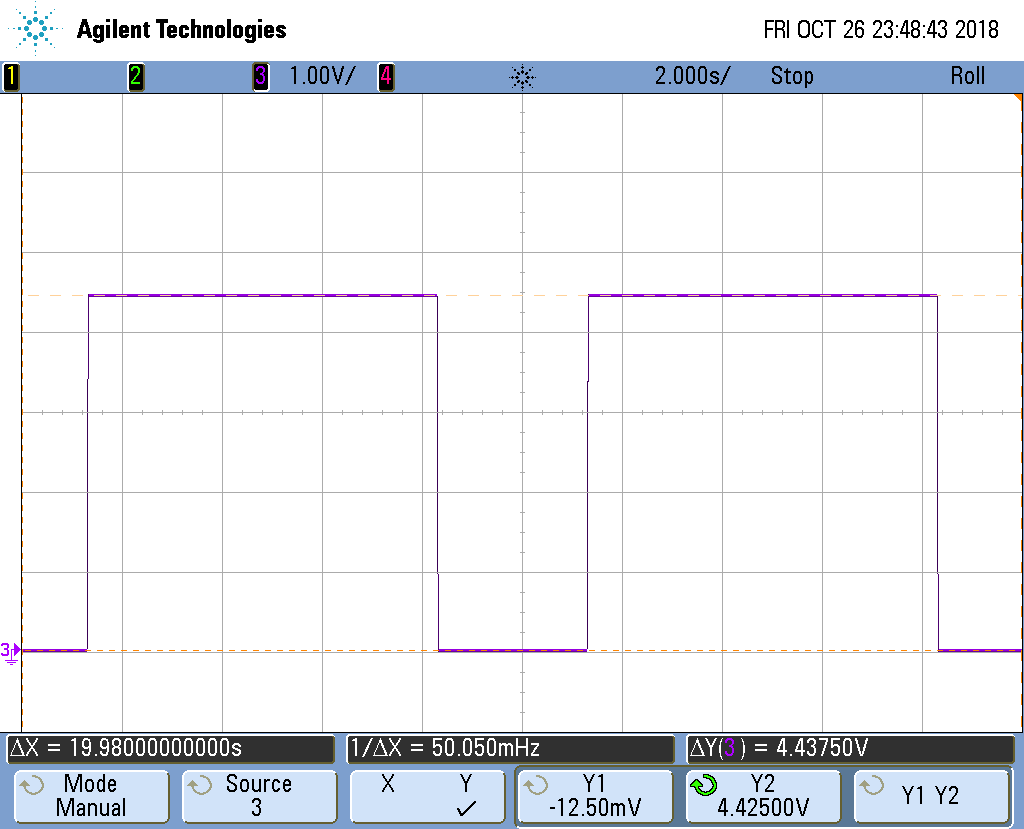
\includegraphics[scale=0.75]{../images/scope_14.png}
	\caption{$V_{in}$ Measurement for $4.5$\si{\volt} Reference}
	\label{fig:scope_14}
\end{figure}

\FloatBarrier

\FloatBarrier

\begin{figure}[h!]
	\centering
	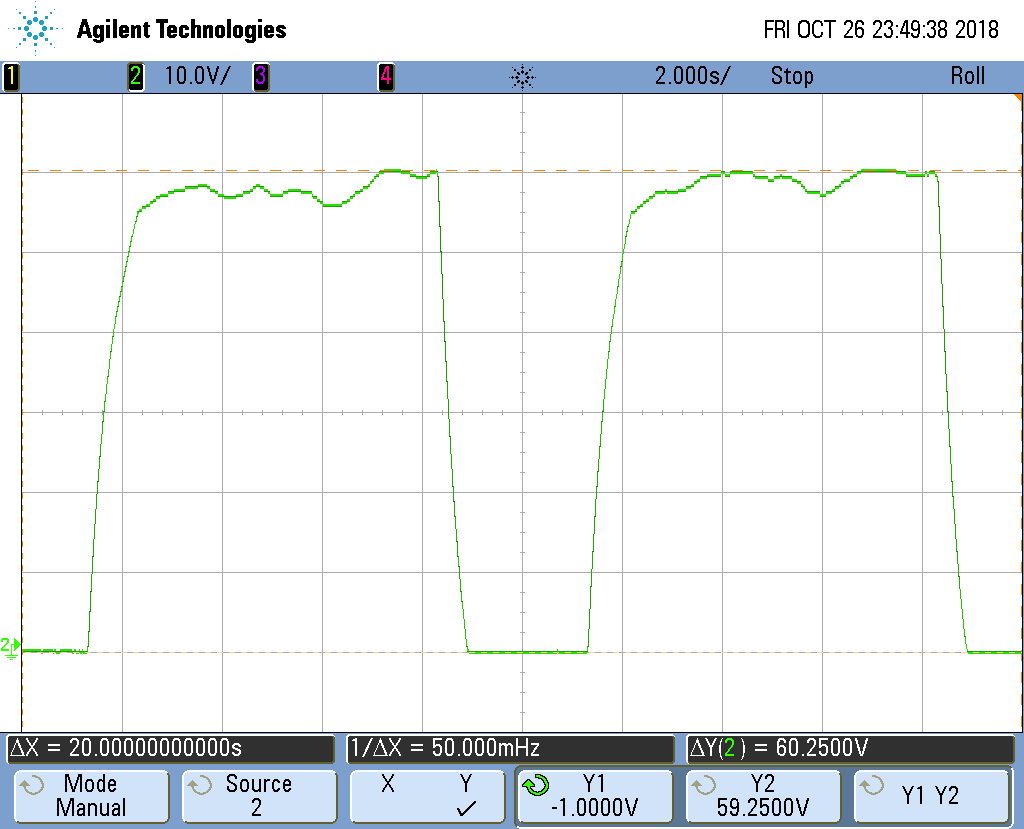
\includegraphics[scale=0.75]{../images/scope_15.png}
	\caption{$V_{out}$ Measurement for $4.5$\si{\volt} Reference}
	\label{fig:scope_15}
\end{figure}

\FloatBarrier

\FloatBarrier

\begin{figure}[h!]
	\centering
	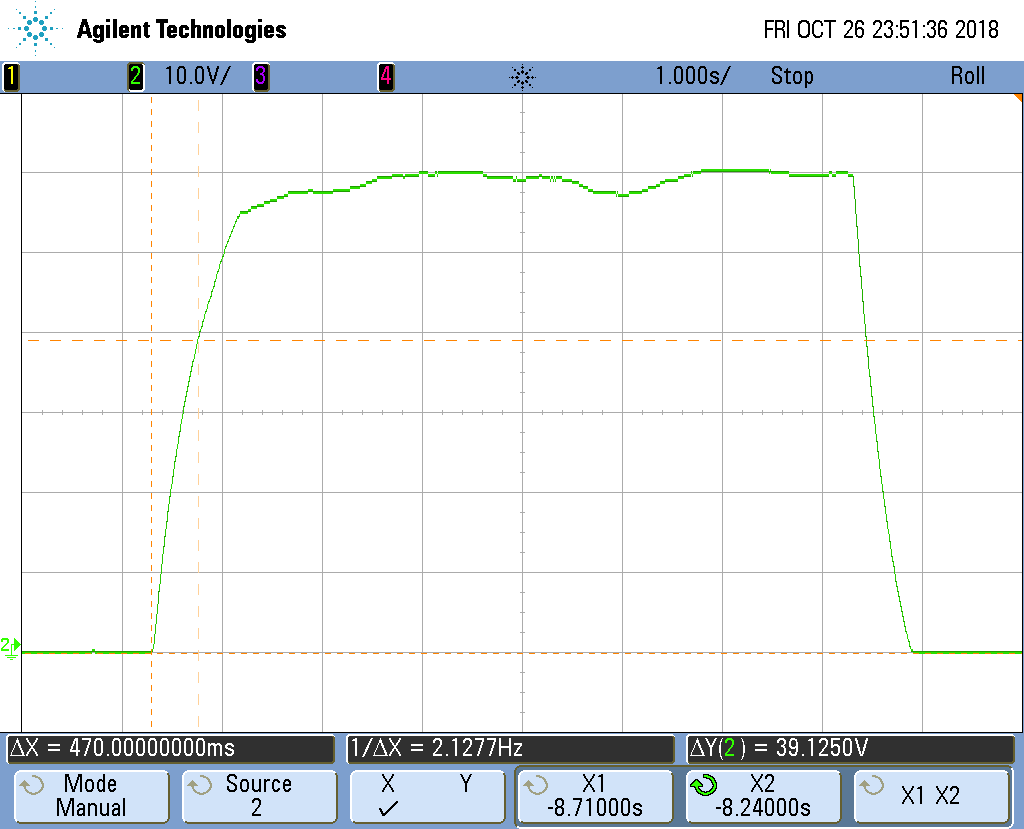
\includegraphics[scale=0.75]{../images/scope_16.png}
	\caption{$\tau$ Measurement for $4.5$\si{\volt} Reference}
	\label{fig:scope_16}
\end{figure}

\FloatBarrier

$C_1$ is determined by applying equation (\ref{eq:steady_state_step}).

\begin{equation}
	\label{eq:solve_for_steady_state}
	C_1 = \frac{ V_{out,ss} }{ V_{in} }
\end{equation}

$C_2$ is determined by observing when the output attains $(1-e^{-1}) \approx 0.63$ of the steady state value, $V_{out,ss}$.

\FloatBarrier

\begin{table}[h!]
	\centering
	\caption{$C_1$ and $C_2$ Results}
	\label{tab:prob_2}
	\csvautotabular{../tables/prob_2.csv}
\end{table}

\FloatBarrier
